\documentclass[12pt, a4paper, oneside]{ctexart}
\usepackage{amsmath, amsthm, amssymb, bm, color, graphicx, geometry, mathrsfs,extarrows, braket, booktabs, array}
\usepackage[colorlinks,linkcolor=red,anchorcolor=blue,citecolor=blue,urlcolor=blue,menucolor=black]{hyperref}
%%%% 设置中文字体 %%%%
\setCJKmainfont{方正新书宋_GBK.ttf}[BoldFont=方正小标宋_GBK, ItalicFont=方正楷体_GBK]
%%%% 设置英文字体 %%%%
\setmainfont{Times New Roman}
\setsansfont{Calibri}
\setmonofont{Consolas}

\linespread{1.4}
%\geometry{left=2.54cm,right=2.54cm,top=3.18cm,bottom=3.18cm}
\geometry{left=1.84cm,right=1.84cm,top=2.18cm,bottom=2.18cm}
\newcounter{problem}  % 问题序号计数器
\newenvironment{problem}[1][]{\stepcounter{problem}\par\noindent\textbf{题目\arabic{problem}. #1}}{\smallskip\par}
\newenvironment{solution}[1][]{\par\noindent\textbf{#1解答. }}{\smallskip\par}  % 可带一个参数表示题号\begin{solution}{题号}
\newenvironment{note}{\par\noindent\textbf{注记. }}{\smallskip\par}

%%%% 图片相对路径 %%%%
\graphicspath{{figure/}} % 当前目录下的figure文件夹, {../figure/}则是父目录的figure文件夹
\setlength{\abovecaptionskip}{-0.2cm}  % 缩紧图片标题与图片之间的距离
\setlength{\belowcaptionskip}{0pt} 

\everymath{\displaystyle} % 默认全部行间公式
\DeclareMathOperator*\uplim{\overline{lim}} % 定义上极限 \uplim_{}
\DeclareMathOperator*\lowlim{\underline{lim}} % 定义下极限 \lowlim_{}
\DeclareMathOperator*{\argmax}{arg\,max}  % \argmin
\DeclareMathOperator*{\argmin}{arg\,min}  % \argmax
\let\leq=\leqslant % 将全部leq变为leqslant
\let\geq=\geqslant % geq同理
\DeclareRobustCommand{\rchi}{{\mathpalette\irchi\relax}}
\newcommand{\irchi}[2]{\raisebox{\depth}{$#1\chi$}} % 使用\rchi将\chi居中

%%%% 一些宏定义 %%%%
\def\bd{\boldsymbol}        % 加粗(向量) boldsymbol
\def\disp{\displaystyle}    % 使用行间公式 displaystyle(默认)
\def\tsty{\textstyle}       % 使用行内公式 textstyle
\def\sign{\text{sign}}      % sign function
\def\wtd{\widetilde}        % 宽波浪线 widetilde
\def\R{\mathbb{R}}          % Real number
\def\N{\mathbb{N}}          % Natural number
\def\Z{\mathbb{Z}}          % Integer number
\def\Q{\mathbb{Q}}          % Rational number
\def\C{\mathbb{C}}          % Complex number
\def\N{\mathbb{N}}          % Natural number
\def\Z{\mathbb{Z}}          % Integer number
\def\E{\mathbb{E}}          % Exception
\def\var{\text{Var}}        % Variance
\def\cov{\text{Cov}}        % Coefficient of Variation
\def\bias{\text{bias}}      % bias
\def\d{\mathrm{d}}          % differential operator
\def\e{\mathrm{e}}          % Euler's number
\def\i{\mathrm{i}}          % imaginary number
\def\re{\mathrm{Re}}        % Real part
\def\im{\mathrm{Im}}        % Imaginary part
\def\res{\mathrm{Res}}      % Residue
\def\L{\mathcal{L}}         % Loss function
\def\wdh{\widehat}          % 宽帽子 widehat
\def\ol{\overline}          % 上横线 overline
\def\ul{\underline}         % 下横线 underline
\def\add{\vspace{1ex}}      % 增加行间距
\def\del{\vspace{-1.5ex}}   % 减少行间距

%%%% 定理类环境的定义 %%%%
\newtheorem{theorem}{定理}

%%%% 基本信息 %%%%
\newcommand{\RQ}{\today} % 日期
\newcommand{\km}{数理统计} % 科目
\newcommand{\bj}{强基数学002} % 班级
\newcommand{\xm}{吴天阳} % 姓名
\newcommand{\xh}{2204210460} % 学号
\newcommand{\id}{50} % 序号

\begin{document}

%\pagestyle{empty}
\pagestyle{plain}
\vspace*{-15ex}
\centerline{\begin{tabular}{*6{c}}
    \parbox[t]{0.25\linewidth}{\begin{center}\textbf{日期}\\ \large \textcolor{blue}{\RQ}\end{center}} 
    & \parbox[t]{0.2\linewidth}{\begin{center}\textbf{科目}\\ \large \textcolor{blue}{\km}\end{center}}
    & \parbox[t]{0.2\linewidth}{\begin{center}\textbf{班级}\\ \large \textcolor{blue}{\bj}\end{center}}
    & \parbox[t]{0.1\linewidth}{\begin{center}\textbf{姓名}\\ \large \textcolor{blue}{\xm}\end{center}}
    & \parbox[t]{0.15\linewidth}{\begin{center}\textbf{学号}\\ \large \textcolor{blue}{\xh}\end{center}}
    & \parbox[t]{0.1\linewidth}{\begin{center}\textbf{序号}\\ \large \textcolor{blue}{\id}\end{center}}
     \\ \hline
\end{tabular}}
\begin{center}
    \zihao{3}\textbf{第七次作业}
\end{center}\vspace{-0.2cm}
% 正文部分
\begin{problem}[(2)]
    令$X$是来自$f(x;\theta) = \theta x^{\theta-1}I_{(0,1)}(x)$的随机变量.

    (a). 设检验$T$是关于$H_0:\theta\leq 1\ vs.\ H_1:\theta > 1$,选取样本量为$2$,拒绝域$C=\{(x_1,x_2):3/4x_1\leq x_2\}$. 求$T$的势函数和检验水平.

    (b). 当检验量为$2$时,求$\alpha = \frac{1}{2}(1-\ln 2)$时关于$H_0:\theta=1\ vs.\ H_1:\theta=2$的MPT.

    (f). 设检验$T$是样本量为$2$下关于$H_0:\theta=1\ vs.\ H_1:\theta=2$,令$\alpha,\beta$分别为第一、二类错误,求检验$T$使得$\max\{\alpha,\beta\}$最小.
\end{problem}
\begin{solution}
    (a). 由于$\pi_T(\theta) = P_\theta(3/4\leq x_2/x_1)$,令$\begin{cases}
        Y_1 = X_1,\\ Y_2=X_2/X_1.
    \end{cases}$于是$\begin{cases}
        X_1=Y_1,\\
        X_2=Y_1Y_2.
    \end{cases}$则$J = Y_1$. 由于$f_{X_1,X_2} = \theta^2(x_1x_2)^{\theta-1}$,通过变量代换可得
    \begin{equation*}
        f_{Y_1,Y_2}(y_1,y_2) = P_{X_1,X_2}(y_1,y_1y_2)y_1 = \theta^2 y_1^{2\theta-1}y_2^{\theta-1}
    \end{equation*}

    当$0 < y_2\leq 1$时,$y_1\in (0,1)$,则$f_{Y_2}(y_2) = \int_0^1\theta^2y_1^{2\theta-1}y_2^{\theta-1}\,\d y_1 = \frac{\theta}{2}y_2^{\theta-1}$.

    当$y_2\geq 1$时,$y_1\in (0,1/y_2)$,则$f_{Y_2}(y_2) = \int_0^{\frac{1}{y_2}}\theta^2y_1^{2\theta-1}y_2^{\theta-1}\,\d y_1 = \frac{\theta}{2}y_2^{-\theta-1}$.

    于是检验函数为$\pi_T(\theta) = P_{\theta}(Y_2\geq 3/4)=\int_{3/4}^1\frac{\theta}{2}y^{\theta-1}\,\d y+\int_1^\infty\frac{\theta}{2}y^{-\theta-1}\,\d y = 1-\frac{1}{2}\left(\frac{3}{4}\right)^{\theta}$,检验水平为$\alpha = \sup_{\theta\leq 1}\pi_T(\theta) = \sup_{\theta \leq 1}1-\frac{1}{2}\left(\frac{3}{4}\right)^\theta = \frac{5}{8}$.

    (b). 由于假设为简单假设,MPT就是SLR检验,$L(\theta) = \theta^2(x_1x_2)^{\theta-1}$,于是$\frac{L(1)}{L(2)} = \frac{1}{4x_1x_2}$,则
    \begin{equation*}
        \alpha=P_{\theta=1}\left[\frac{L(1)}{L(2)}< k^*\right]= P_{\theta = 1}\left[X_1X_2> \frac{1}{4k^*}\right] = P_{\theta = 1}[X_1X_2> k']
    \end{equation*}
    令$\begin{cases}
        Y_1 = X_1,\\
        Y_2 = X_1X_2.
    \end{cases}\Rightarrow \begin{cases}
        x_1 = y_1,\\
        x_2 = y_2/y_1.
    \end{cases}$则$J = \frac{1}{y_1}$,由于$\theta = 1$,则$X_1,X_2\overset{iid}{\sim}I_{(0,1)}$,于是$f_{Y_1,Y_2}(y_1,y_2) = \frac{1}{y_1}$,则
    \begin{equation*}
        f_{Y_2}(y_2) = \int_{y_2}^1\frac{1}{y_1}\,\d y_1 = -\log y_2
    \end{equation*}
    则
    \begin{equation*}
        \frac{1}{2}+\frac{1}{2}\log\frac{1}{2}=\alpha = P_{\theta=1}(x_1x_2> k') = P_{\theta = 1}(Y_2> k') = \int_{k'}^1-\log y\,\d y = 1+k'\log k'-k'
    \end{equation*}
    故$k' = 1/2$,MPT为拒绝$H_0$当且仅当$X_1X_2> 1/2$.
\end{solution}
\begin{problem}[(4)]设$X$来自分布$f(x;\theta) = \theta x^{\theta-1}I_{(0,1)}(x)$,其中$\theta >0$.

    (a). 设假设$H_0:\theta \leq 1\ vs.\ H_1:\theta > 1$,求出拒绝域$C=\{x:x\geq 1/2\}$的势函数和检验水平.

    (b). 求解关于$H_0:\theta=2\ vs.\ H_1:\theta=1$检验水平为$\alpha$的MPT.

    (d). 求解关于$H_0:\theta\geq 2\ vs.\ H_1:\theta <  2$检验水平为$\alpha$的UMPT.

    (e). 对于所有关于$H_0:\theta = 2\ vs.\ H_1:\theta=1$的简单似然比检验,求解检验最小化$\alpha+\beta$,其中$\alpha,\beta$为犯第一类和第二类错误的概率.

    (f). 求检验水平为$\alpha$的GLR,关于$H_0:\theta=1\ vs.\ H_1:\theta\neq 1$.
\end{problem}
\begin{solution}
    (a). 势函数:$\pi_{T}(\theta)j = P_{\theta}\left[X\geq \frac{1}{2}\right] = \int_{\frac{1}{2}}^1\theta x^{\theta-1}\,\d x=1-\left(\frac{1}{2}\right)^\theta$,\add \\
    检验水平:$\alpha = \sup_{\theta\leq 1}\pi_T(\theta) = \sup_{\theta\leq 1}1-\left(\frac{1}{2}\right)^\theta = \frac{1}{2}$.\add 

    (b). 由于简单假设中MPT是SLR检验,则$L(\theta) = f(x) = \theta x^{\theta-1}$,于是$L_0/L_1 = L(2) / L(1) = 2x$,则
    \begin{equation*}
        \alpha = P_{\theta=2}\left(\frac{L_0}{L_1}<k^*\right)= P_{\theta=2}(2x<k^*) = P_{\theta=2}(x < k') = \int_0^{k'}2x\,\d x\Rightarrow k'=\sqrt{\alpha}
    \end{equation*}
    于是,MPT的拒绝域为$C=\{x:x<\sqrt{\alpha}\}$.\add

    (d). 由于$f(x;\theta) = \theta\exp\{(\theta-1)\log x\}$,于是$T = \log X$,$c(\theta) = \theta-1$是关于$\theta$单调函数,则
    \begin{equation*}
        \alpha  = P_{\theta=2}[\log x < k^*] = P_{\theta=2}[x<k'] = \int_0^{k'}2x\,\d x = k'^2\Rightarrow k' = \sqrt{\alpha}
    \end{equation*}
    于是UMPT的拒绝域为$C = \{x:x < \sqrt{\alpha}\}$.

    (e). 

    (f). 由于$L(\theta) = \theta x^{\theta -1}$,$\frac{\d L(\theta)}{\d \theta} = x^{\theta-1}(1+\theta \log x)$,则$\theta = -\frac{1}{\log x}$时取到最大值,则$\sup_{\theta > 0}L(\theta) = -\frac{1}{\log x}x^{-\frac{1}{\log x}-1}$,$L(1) = 1$,于是
    \begin{equation*}
        \lambda = \frac{L(1)}{\sup_{\theta > 0}L(\theta)} = -x^{\frac{1}{\log x}+1}\log x
    \end{equation*}
    则拒绝$H$当且仅当$-x^{\frac{1}{\log x}+1}\log x < \lambda_0$,令$y=-\log x$,则$x=\e^{-y},\ y\in(0,\infty)$,令
    \begin{equation*}
        g(y) = -x^{\frac{1}{\log x}+1}\log x = -\left(\e^{-y}\right)^{1-\frac{1}{y}}(-y) = y\e^{1-y}
    \end{equation*}
    则$g'(y) = (1-y)\e^{1-y}$,当$y=1$时,$g(y)$有最大值,分两类情况讨论:

    1. $0<y<1$即$\e^{-1}<x<1$时,$g(y)$单调递增,则$g(y) < \lambda_0$等价于$y<k$则
    \begin{equation*}
        \alpha = P_{\theta = 1}[y<k] = \int_0^k\e^{-y}\,\d y = 1-\e^{-k}\Rightarrow k = -\log (1-\alpha)
    \end{equation*}
    于是该部分的拒绝域为$C_0 = \{y: 0<y<\min\{1, k\}\} = \{x:\max\{\e^{-1}, 1-\alpha\} < x < 1\}$.

    2. $y > 1$即$0< x < \e^{-1}$时,$g(y)$单调递减,则$g(y) < \lambda_0$等价于$y > k$则
    \begin{equation*}
        \alpha = P_{\theta = 1}[y > k] = \int_k^\infty \e^{-y}\,\d y = \e^{-k}\Rightarrow k = -\log \alpha
    \end{equation*}
    于是该部分的拒绝域为$C_1 = \{y: y > \max\{1, -\log \alpha\}\} = \{x: 0 < x < \min(\alpha, \e^{-1})\}$.

    综上,GLR检验水平为$\alpha$的拒绝域为$C = C_0\cup C_1 = (0,\min\{\alpha,\e^{-1}\})\cup (\max\{\e^{-1},1-\alpha\}, 1)$.
\end{solution}
\begin{problem}[(中文书7)]
    设样本量为$1$,$X\sim \theta x^{\theta - 1}I_{(0,1)}(x)$,统计假设$H_0:\theta = 1\ vs. H_1:\theta = 2$,若拒绝域为$C = \{x:x\geq c\}$,确定$c$使得$\alpha+2\beta$最小,并求出最小值,$\alpha,\beta$为犯第一类和第二类错误的概率.
\end{problem}

% 下面给一些功能的写法
\iffalse
% 图片模板
\centerline{
    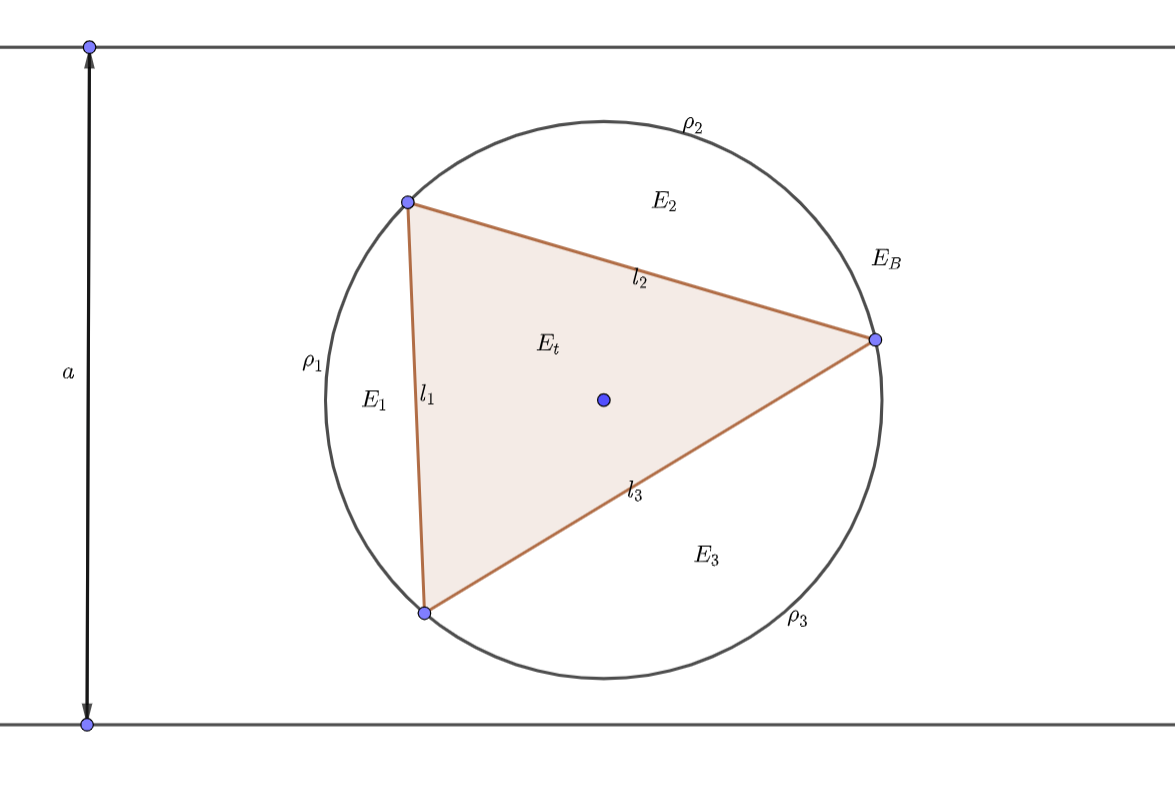
\includegraphics[width=0.8\textwidth]{figure.png}
}
% 表格模板
\renewcommand\arraystretch{0.8} % 设置表格高度为原来的0.8倍
\begin{table}[!htbp] % table标准
    \centering % 表格居中
    \begin{tabular}{p{1cm}<{\centering}p{1cm}<{\centering}p{3cm}<{\centering}p{5cm}<{\centering}} % 设置表格宽度
    %\begin{tabular}{cccc}
        \toprule
        $x_i$ & $f[x_1]$ & $f[x_i,x_{i+1}]$ & $f[x_i,x_{i+1},x_{i+2}]$ \\
        \midrule
        $x_0$ & $f(x_0)$ &                  &                          \\
        $x_0$ & $f(x_0)$ & $f'(x_0)$        &                          \\
        $x_0$ & $f(x_1)$ & $\frac{f(x_1)-f(x_0)}{x_1-x_0}$ & $\frac{f(x_1)-f(x_0)}{(x_1-x_0)^2}-\frac{f'(x_0)}{x_1-x_0}$\\
        \bottomrule
    \end{tabular}
\end{table}

\def\Log{\text{Log}} % 一个简单的宏定义
$\Log$ % 调用方法
\fi

\end{document}